\documentclass[11pt,compress,t,notes=noshow, xcolor=table]{beamer}

% graphicx and color are loaded via lmu-lecture.sty
% maxwidth is the original width if it is less than linewidth
% otherwise use linewidth (to make sure the graphics do not exceed the margin)
% TODO: Remove once cleared to be superfluous
% \makeatletter
% \def\maxwidth{ %
%   \ifdim\Gin@nat@width>\linewidth
%     \linewidth
%   \else
%     \Gin@nat@width
%   \fi
% }
% \makeatother

% ---------------------------------%
% latex-math dependencies, do not remove:
% - mathtools
% - bm
% - siunitx
% - dsfont
% - xspace
% ---------------------------------%

%--------------------------------------------------------%
%       Language, encoding, typography
%--------------------------------------------------------%

\usepackage[english]{babel}
\usepackage[utf8]{inputenc} % Enables inputting UTF-8 symbols
% Standard AMS suite (loaded via lmu-lecture.sty)

% Font for double-stroke / blackboard letters for sets of numbers (N, R, ...)
% Distribution name is "doublestroke"
% According to https://mirror.physik.tu-berlin.de/pub/CTAN/fonts/doublestroke/dsdoc.pdf
% the "bbm" package does a similar thing and may be superfluous.
% Required for latex-math
\usepackage{dsfont}

% bbm – "Blackboard-style" cm fonts (https://www.ctan.org/pkg/bbm)
% Used to be in common.tex, loaded directly after this file
% Maybe superfluous given dsfont is loaded
% TODO: Check if really unused?
% \usepackage{bbm}

% bm – Access bold symbols in maths mode - https://ctan.org/pkg/bm
% Required for latex-math, preferred over \boldsymbol
% https://tex.stackexchange.com/questions/3238/bm-package-versus-boldsymbol
\usepackage{bm}

% pifont – Access to PostScript standard Symbol and Dingbats fonts
% Used for \newcommand{\xmark}{\ding{55}, which is never used
% aside from lecture_advml/attic/xx-automl/slides.Rnw
% \usepackage{pifont}

% Quotes (inline and display), provdes \enquote
% https://ctan.org/pkg/csquotes
\usepackage{csquotes}

% Adds arg to enumerate env, technically superseded by enumitem according
% to https://ctan.org/pkg/enumerate
% Replace with https://ctan.org/pkg/enumitem ?
% Even better: enumitem is not really compatible with beamer and breaks all sorts of things
% particularly the enumerate environment. The enumerate package also just isn't required
% from what I can tell so... don't re-add it I guess?
% \usepackage{enumerate}

% Line spacing - provides \singlespacing \doublespacing \onehalfspacing
% https://ctan.org/pkg/setspace
% \usepackage{setspace}

% mathtools – Mathematical tools to use with amsmath
% https://ctan.org/pkg/mathtools?lang=en
% latex-math dependency according to latex-math repo
\usepackage{mathtools}

% Maybe not great to use this https://tex.stackexchange.com/a/197/19093
% Use align instead -- TODO: Global search & replace to check, eqnarray is used a lot
% $ rg -f -u "\begin{eqnarray" -l | grep -v attic | awk -F '/' '{print $1}' | sort | uniq -c
%   13 lecture_advml
%   14 lecture_i2ml
%    2 lecture_iml
%   27 lecture_optimization
%   45 lecture_sl
\usepackage{eqnarray}
% For shaded regions / boxes
% Used sometimes in optim
% https://www.ctan.org/pkg/framed
\usepackage{framed}

%--------------------------------------------------------%
%       Cite button (version 2024-05)
%--------------------------------------------------------%

% Superseded by style/ref-buttons.sty, kept just in case these don't work out somehow.

% Note this requires biber to be in $PATH when running,
% telltale error in log would be e.g. Package biblatex Info: ... file 'authoryear.dbx' not found
% aside from obvious "biber: command not found" or similar.
% Tried moving this to lmu-lecture.sty but had issues I didn't quite understood,
% so it's here for now.

\usepackage{hyperref}

% Only try adding a references file if it exists, otherwise
% this would compile error when references.bib is not found
% NOTE: Bibliography packages (usebib, biblatex) are now loaded by ref-buttons.sty when needed
% This keeps all bibliography-related setup in one place

% Legacy \citelink command removed - superseded by ref-buttons.sty

%--------------------------------------------------------%
%       Displaying code and algorithms
%--------------------------------------------------------%

% Reimplements verbatim environments: https://ctan.org/pkg/verbatim
% verbatim used sed at least once in
% supervised-classification/slides-classification-tasks.tex
% Removed since code should not be put on slides anyway
% \usepackage{verbatim}

% Both used together for algorithm typesetting, see also overleaf: https://www.overleaf.com/learn/latex/Algorithms
% algorithmic env is also used, but part of the bundle:
%   "algpseudocode is part of the algorithmicx bundle, it gives you an improved version of algorithmic besides providing some other features"
% According to https://tex.stackexchange.com/questions/229355/algorithm-algorithmic-algorithmicx-algorithm2e-algpseudocode-confused
\usepackage{algorithm}
\usepackage{algpseudocode}

%--------------------------------------------------------%
%       Tables
%--------------------------------------------------------%

% multi-row table cells: https://www.namsu.de/Extra/pakete/Multirow.html
% Provides \multirow
% Used e.g. in evaluation/slides-evaluation-measures-classification.tex
\usepackage{multirow}

% colortbl: https://ctan.org/pkg/colortbl
% "The package allows rows and columns to be coloured, and even individual cells." well.
% Provides \columncolor and \rowcolor
% \rowcolor is used multiple times, e.g. in knn/slides-knn.tex
\usepackage{colortbl}

% long/multi-page tables: https://texdoc.org/serve/longtable.pdf/0
% Not used in slides
% \usepackage{longtable}

% pretty table env: https://ctan.org/pkg/booktabs
% Is used
% Defines \toprule
\usepackage{booktabs}

%--------------------------------------------------------%
%       Figures: Creating, placing, verbing
%--------------------------------------------------------%

% wrapfig - Wrapping text around figures https://de.overleaf.com/learn/latex/Wrapping_text_around_figures
% Provides wrapfigure environment -used in lecture_optimization
\usepackage{wrapfig}

% Sub figures in figures and tables
% https://ctan.org/pkg/subfig -- supersedes subfigure package
% Provides \subfigure
% \subfigure not used in slides but slides-tuning-practical.pdf errors without this pkg, error due to \captionsetup undefined
\usepackage{subfig}

% Actually it's pronounced PGF https://en.wikibooks.org/wiki/LaTeX/PGF/TikZ
\usepackage{tikz}

% No idea what/why these settings are what they are but I assume they're there on purpose
\usetikzlibrary{shapes,arrows,automata,positioning,calc,chains,trees, shadows}
\tikzset{
  %Define standard arrow tip
  >=stealth',
  %Define style for boxes
  punkt/.style={
    rectangle,
    rounded corners,
    draw=black, very thick,
    text width=6.5em,
    minimum height=2em,
    text centered},
  % Define arrow style
  pil/.style={
    ->,
    thick,
    shorten <=2pt,
    shorten >=2pt,}
}


% textpos package to allow absolute placement of environments like figures
% See e.g. https://datumorphism.leima.is/til/programming/latex-beamer-textblock-position/
%  - absolute: Enables absolute positioning mode where coordinates are measured from the top-left corner of the page/frame, rather than relative to the current text position.
%  - overlay: Makes the positioned content behave as an overlay that doesn't affect the normal text flow or spacing. Without this, positioned elements could interfere with the document's layout.
% 
%   The \textblock* environment creates a text block at absolute coordinates:
% 
%   \begin{textblock*}{\linewidth}(0cm,4cm) % (x,y) from top-left of frame
%     \imageC[1]{figure/cov_funs/cov_matern.pdf}
%   \end{textblock*}
\usepackage[absolute,overlay]{textpos}

%--------------------------------------------------------%
%       Beamer setup and custom macros & environments
%--------------------------------------------------------%

% Main sty file for beamer setup (layout, style, lecture page numbering, etc.)
% For long-term maintenance, this may me refactored into a more modular set of .sty files
\usepackage{../../style/lmu-lecture-new}
% Custom itemize wrappers, itemizeS, itemizeL, etc

% Used regularly
\let\code=\texttt

% Not sure what/why this does
\setkeys{Gin}{width=0.9\textwidth}

% -- knitr leftovers --
% These may be used by knitr/R Markdown workflows in other lectures
\makeatletter
\def\maxwidth{ %
  \ifdim\Gin@nat@width>\linewidth
    \linewidth
  \else
    \Gin@nat@width
  \fi
}
\makeatother

% Define colors for syntax highlighting (may be used by knitr)
\definecolor{fgcolor}{rgb}{0.345, 0.345, 0.345}
\definecolor{shadecolor}{rgb}{.97, .97, .97}

% knitr code output environment
\newenvironment{knitrout}{}{}

\newcommand{\citebutton}[2]{%
\beamergotobutton{\href{#2}{#1}}%
}

\newcommand{\ques}{\textbf{\textcolor{red}{Question:  }}}
\newcommand{\questionssofar}{\begin{frame}\frametitle{Any questions?}\end{frame}}

\newcommand\warning{%
 \makebox[1.4em][c]{%
 \makebox[0pt][c]{\raisebox{.1em}{\scriptsize!}}%
 \makebox[0pt][c]{\color{red}\normalsize$\bigtriangleup$}}}%

% Can't find a reason why common.tex is not just part of this file?
% This file is included in slides and exercises

% Rarely used fontstyle for R packages, used only in 
% - forests/slides-forests-benchmark.tex
% - exercises/single-exercises/methods_l_1.Rnw
% - slides/cart/attic/slides_extra_trees.Rnw
\newcommand{\pkg}[1]{{\fontseries{b}\selectfont #1}}

% Spacing helpers, used often (mostly in exercises for \dlz)
\newcommand{\lz}{\vspace{0.5cm}} % vertical space (used often in slides)
\newcommand{\dlz}{\vspace{1cm}}  % double vertical space (used often in exercises, never in slides)
\newcommand{\oneliner}[1] % Oneliner for important statements, used e.g. in iml, algods
{\begin{block}{}\begin{center}\begin{Large}#1\end{Large}\end{center}\end{block}}

% Don't know if this is used or needed, remove?
% textcolor that works in mathmode
% https://tex.stackexchange.com/a/261480
% Used e.g. in forests/slides-forests-bagging.tex
% [...] \textcolor{blue}{\tfrac{1}{M}\sum^M_{m} [...]
% \makeatletter
% \renewcommand*{\@textcolor}[3]{%
%   \protect\leavevmode
%   \begingroup
%     \color#1{#2}#3%
%   \endgroup
% }
% \makeatother



% custom packages
\usepackage{subfig}
\usepackage{psfrag}
\usepackage{algorithm}
\usepackage{algpseudocode}
\usepackage{eqnarray}
\usepackage{arydshln}
\usepackage{tabularx}
\usepackage{placeins}
\usepackage{tikz}
\usepackage{setspace}
\usepackage{colortbl}
\usepackage{mathtools}
\usepackage{wrapfig}
\usepackage{listings}

\usepackage{framed}
\makeatletter
\newenvironment{kframe}{%
 \def\at@end@of@kframe{}%
 \ifinner\ifhmode%
  \def\at@end@of@kframe{\end{minipage}}%
  \begin{minipage}{\columnwidth}%
 \fi\fi%
 \def\FrameCommand##1{\hskip\@totalleftmargin \hskip-\fboxsep
 \colorbox{shadecolor}{##1}\hskip-\fboxsep
     % There is no \\@totalrightmargin, so:
     \hskip-\linewidth \hskip-\@totalleftmargin \hskip\columnwidth}%
 \MakeFramed {\advance\hsize-\width
   \@totalleftmargin\z@ \linewidth\hsize
   \@setminipage}}%
 {\par\unskip\endMakeFramed%
 \at@end@of@kframe}
\makeatother

\usepackage{tcolorbox}
\usepackage{dsfont}
\usepackage{tikz}

\definecolor{texblue}{rgb}{0, 0, 1}
\def\myblue#1{\textcolor{texblue}{#1}}

\newcommand{\vocab}{\mathcal{V}}
\newcommand{\probs}{\boldsymbol{\phi}}

\tikzset{
  invisible/.style={opacity=0, text opacity=0},
  visible on/.style={alt={#1{}{invisible}}},
  alt/.code args={<#1>#2#3}{\alt<#1>{\pgfkeysalso{#2}}{\pgfkeysalso{#3}}},
  pf pt/.style={circle, fill=#1, inner sep=1.6pt},
  pf seq/.style={font=\footnotesize, text=#1, anchor=south, inner sep=2pt},
  pf num/.style={font=\scriptsize, text=#1, inner sep=1pt},
  pf map/.style={->, thick, draw=#1, shorten <=2pt, shorten >=2pt},
  pf fibre/.style={rounded corners=4pt, fill=#1!7, draw=#1!40},
}


% Run bibliography entries together instead of breaking after each block
\setbeamertemplate{bibliography entry title}{}
\setbeamertemplate{bibliography entry location}{}
\setbeamertemplate{bibliography entry note}{}

% Numbered labels [1], [2] instead of the little paper icon
\setbeamertemplate{bibliography item}{\insertbiblabel}

% ToC
\AtBeginSection[]{
	\begin{frame}[noframenumbering, plain]
	\frametitle{Outline}
	\setcounter{tocdepth}{1}
	\tableofcontents[currentsection]
\end{frame}
}

\title{Deep Learning for NLP II}

\begin{document}

\titlemeta{
Tokenization
}{}{
figure/tokenization-title.png
}{
\item Motivation for subword tokenization
\item Overview of BPE and Unigram
\item Open questions in tokenization
}

% ------------------------------------------------------------------------------

\begin{frame}{Outline}
\tableofcontents
\end{frame}

% ==============================================================================
% MOTIVATION & CONTEXT
% ==============================================================================


\section{Subword Tokenization Basics}

\begin{frame}{Motivation}

\vspace*{\stretch{1}}

\begin{itemize}

\item An LLM cannot simply digest the input text as is (infinite number of possible input texts)

\item We need to map the input text to a sequence of units that the LLM ``knows'' (i.e., that correspond to fixed input representations)

\item This step is commonly referred to as \textbf{tokenization}, and the units known to the LLM as \textbf{tokens}

\end{itemize}

\vspace*{\stretch{1}}

      \centering

      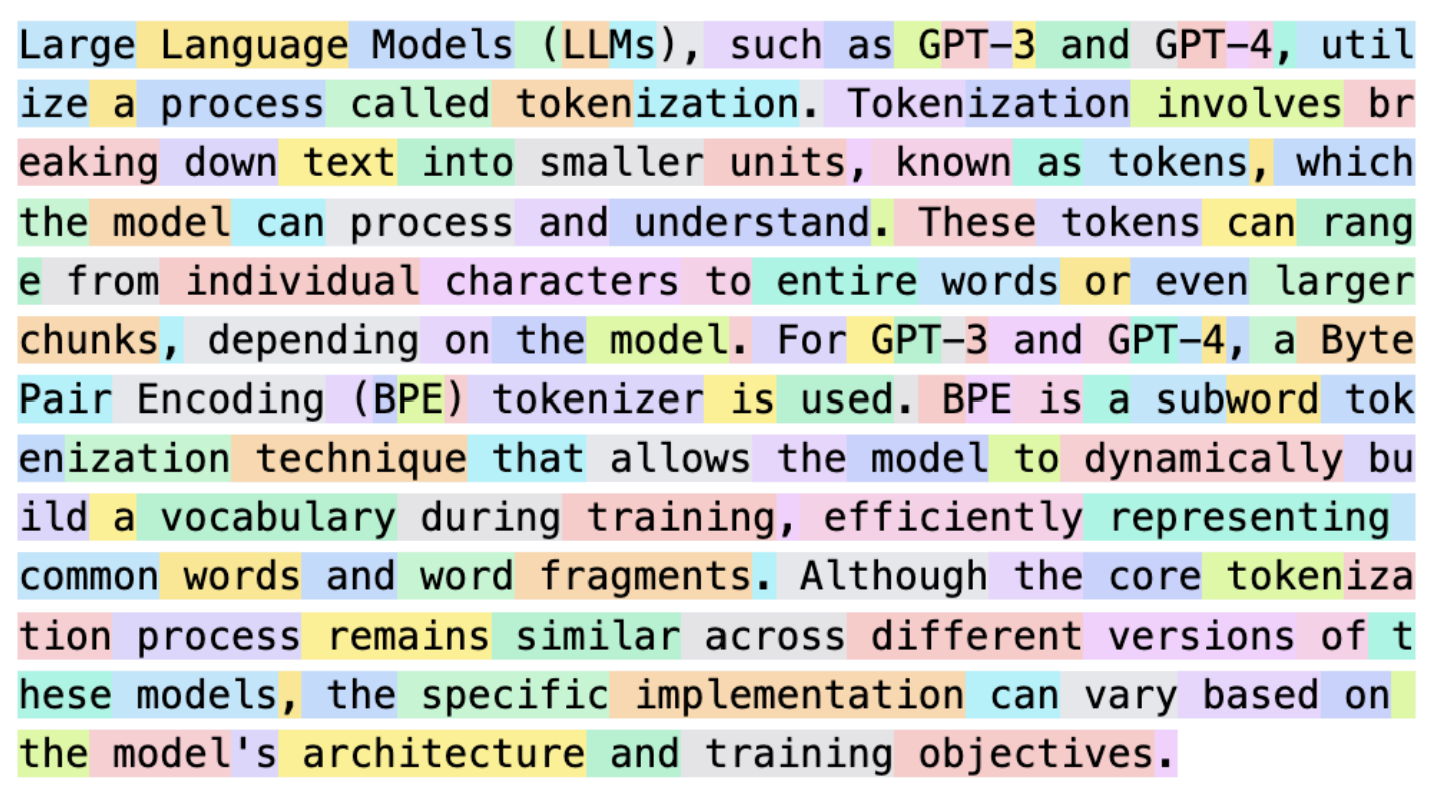
\includegraphics[width=0.6\textwidth]{figure/tokenization-title.png}


\vspace*{\stretch{1}}

\end{frame}


\begin{frame}{Try It Yourself!}

\vfill

\begin{itemize}
\item Experiment with different types of input (e.g., different languages)
\item What do you observe?
\item How would you characterize the generated tokens?
\end{itemize}

\vfill

\centering

      
\includegraphics[width=0.3\textwidth]{figure/qr_gpt_tok.png}\\
\url{https://platform.openai.com/tokenizer}

\vfill

\end{frame}

\begin{frame}{Types of Tokenization}

\vfill

\begin{itemize}
\item \textbf{Word-level} tokenization
\item \textbf{Character-level} (or \textbf{byte-level}) tokenization
\item \textbf{Subword-level} tokenization $\leftarrow$ used by most LLMs
\end{itemize}

\vfill

\end{frame}



\begin{frame}{Word-Level Tokenization}

\vfill

\begin{itemize}
\item Idea: split the input text into a sequence of \textbf{words}
\item Widely used in pre-LLM NLP (e.g., static word embeddings)
\item Pros:
\begin{itemize}
\item Relatively simple to implement
\item Exact lexical representations
\end{itemize}
\item Cons:
\begin{itemize}
\item Large LLM vocabularies are computationally very expensive
\item \textbf{Heaps' law}: full coverage of all words impossible $\rightarrow$ many out-of-vocabulary (OOV) words

\end{itemize}
\end{itemize}

\vfill


\end{frame}


\begin{frame}{Zipf's Law Recap}

\vfill

\begin{itemize}
\item Mathematical form (simplified): $p(w_n) \propto 1 / n$
\begin{itemize}
\item $p$: relative frequency of a word
\item $w_n$: word at frequency rank $n$ in a text
\end{itemize}

\item Intuition: the second most common word occurs about half as often as the first, the third about a third as often, etc.
\end{itemize}

\vfill

\centering

      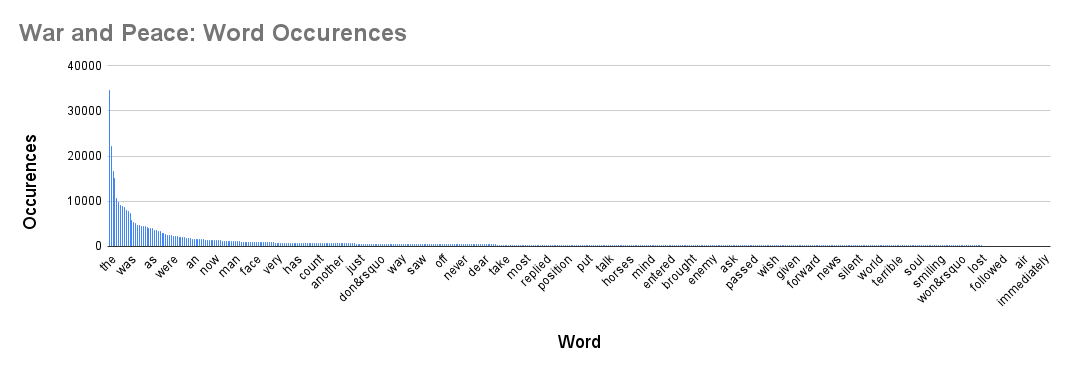
\includegraphics[width=\textwidth]{figure/zipf.png}
\vfill


\end{frame}



\begin{frame}{Heaps' Law}

\vfill

\begin{itemize}
\item Mathematical form: $V(n) = K n^\beta$
\begin{itemize}
\item $V$: vocabulary size (i.e., number of distinct word types)
\item $n$: corpus size (i.e., number of word tokens)
\item $K$, $\beta$: parameters (typically $10 < K < 100$, $0.4 < \beta < 0.6$)

\end{itemize}
\item Intuition: the more text you read, the fewer new words you encounter, but you never stop encountering them
\end{itemize}

\medskip

\centering

      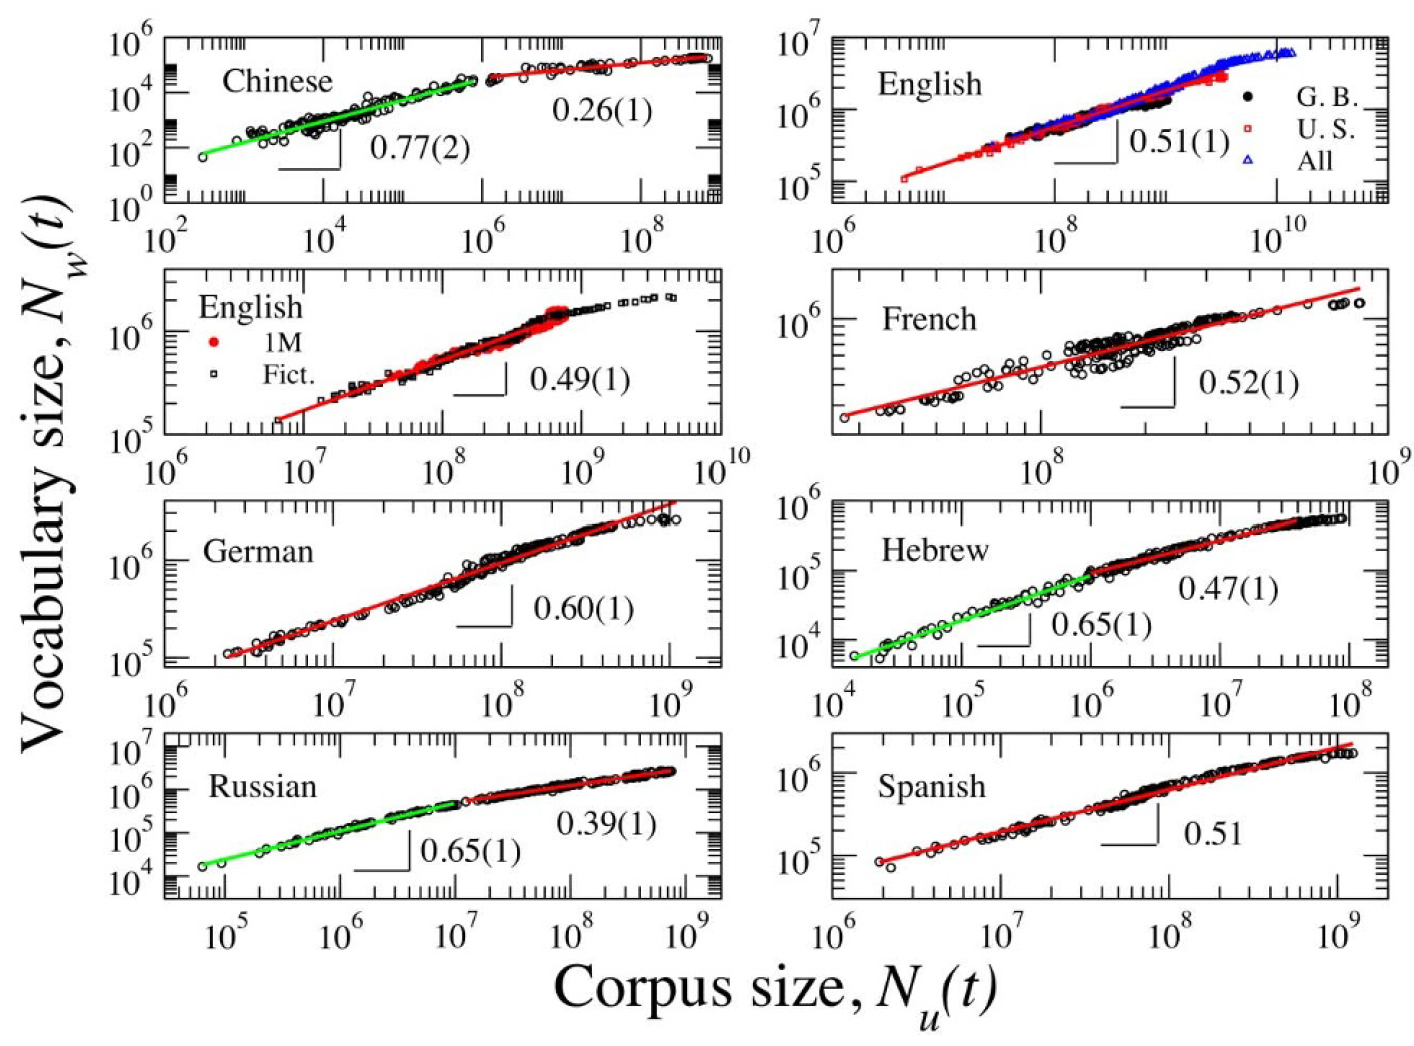
\includegraphics[width=0.55\textwidth]{figure/heap.png}
\vfill


\end{frame}

\begin{frame}{Character-Level Tokenization}

\vfill

\begin{itemize}
\item Idea: split the input text into a sequence of \textbf{characters} (or \textbf{bytes})
\item Pros:
\begin{itemize}
\item Simple to implement
\item Leads to small token vocabularies
\end{itemize}
\item Cons:
\begin{itemize}
\item Lexical representations become a function of characters
\item Difficult to train in practice

\end{itemize}
\end{itemize}

\vfill


\end{frame}



\begin{frame}{Subword-Level Tokenization}

\vfill

\begin{itemize}
\item Idea: split the input text into a mixed sequence of \textbf{words}, \textbf{subwords}, and \textbf{characters} (or \textbf{bytes})
\item Pros:
\begin{itemize}
\item Relatively small token vocabularies (30K to 100K tokens)
\item Exact lexical representations for frequent words
\item Less frequent words represented as a (typically short) sequence of subwords and characters
\end{itemize}
\item Cons:
\begin{itemize}
\item Most complex tokenization approach
\end{itemize}

\end{itemize}

\vfill

\end{frame}

\begin{frame}{Common Subword-Level Tokenizers}

\vfill

\begin{itemize}
\item \textbf{Byte-pair encoding (BPE)} \citebutton{Sennrich et al. (2016)\cite{sennrich-etal-2016-neural}}{https://aclanthology.org/P16-1162/}: GPT, Llama, Qwen 
\item \textbf{Unigram} \citebutton{Kudo (2018)\cite{kudo-2018-subword}}{https://aclanthology.org/P18-1007/}: ALBERT, XLNet, T5

\item Two key questions:
\begin{itemize}
\item Training: how to determine the vocabulary of tokens?
\item Inference: how to segment texts into tokens?

\end{itemize}

\end{itemize}



\vfill

\end{frame}


\begin{frame}{Notation}

\vfill


\begin{itemize}
\item $\mathbf{s} = \langle s_1, s_2, \dots \rangle$: sequence of characters/bytes, such that $s_t \in \Sigma$ for a base alphabet $\Sigma$
\item $\mathbf{v} = \langle v_1, v_2, \dots \rangle$: sequence of \textbf{tokens}, such that $v_t \in \vocab$ for a finite set $\vocab$ called \textbf{vocabulary}
\item $h: \Sigma^* \to \vocab^*$: \textbf{tokenization function}
\item $\mathbf{s}$ can be reconstructed from $\mathbf{v}$ via a \textbf{detokenization function} $g: \vocab^* \to \Sigma^* $ (simple mapping like string concatenation)
\item $g$ is generally non-injective: there can be (and often are) multiple valid $\mathbf{v}$ for which $g$ would lead to the same $\mathbf{s}$
\item $\mathcal{T}_{\vocab}(\mathbf{s}) = g^{-1}(\mathbf{s}) = \{ \mathbf{v} \in \vocab^* : g(\mathbf{v}) = \mathbf{s}\}$: set of all valid token sequences that detokenize to $\mathbf{s}$
\item $h(\mathbf{s})$ is the \textbf{canonical tokenization}, whereas $\mathbf{v} \in \mathcal{T}_{\vocab}(\mathbf{s})$ with $\mathbf{v} \neq h(\mathbf{s})$ are \textbf{non-canonical tokenizations}
\end{itemize}

\vfill


\end{frame}


\begin{frame}{Example}

\vfill

\begin{itemize}
\item $\vocab = \{ \texttt{h},\texttt{a}, \texttt{t}, \texttt{ha}, \texttt{at} \}$
\item $h(\textit{hat}) = \langle \texttt{ha}, \texttt{t}\rangle$
\item $g(\langle \texttt{ha}, \texttt{t}\rangle) = \textit{hat} $
\item $\mathcal{T}_{\vocab}(\textit{hat}) = \{ \langle \texttt{h}, \texttt{a}, \texttt{t}\rangle, \langle \texttt{ha}, \texttt{t}\rangle, \langle \texttt{h}, \texttt{at}\rangle \}$
\item $\langle \texttt{ha}, \texttt{t}\rangle$ is the canonical tokenization
\item $\langle \texttt{h}, \texttt{a}, \texttt{t}\rangle$ is a non-canonical tokenization
\end{itemize}

\vfill

\end{frame}



\section{Overview of BPE}



\begin{frame}{BPE Training}

\vfill

\begin{itemize}
\item Originally a \textbf{text compression algorithm}
\item Initialization: 
\begin{itemize}
\item Base vocabulary: $\vocab = \Sigma$
\item Apply \textbf{normalization} and \textbf{pretokenization} (e.g., split on whitespace)
\item \textbf{Bottom-up} approach: Each $\mathbf{s}$ starts as its character sequence $\mathbf{v} = \langle s_{1}, \dots, s_{|\mathbf{s}|} \rangle$
\end{itemize}
\item Repeat until $|\vocab|$ reaches the target size:
  \begin{itemize}
  \item Count adjacent token pairs $\langle u, w \rangle$ in the corpus
  \item Take the most frequent pair $(u^*, w^*)$, add the new token $u^*w^*$ to $\vocab$, and record the merge rule $(u^*, w^*) \to u^*w^*$
  \item Replace every occurrence of $\langle u^*, w^* \rangle$ in the corpus by $u^*w^*$
  \end{itemize}
\item Output: vocabulary $\vocab$ and an ordered list of merge rules
\end{itemize}

\vfill

\end{frame}


\begin{frame}{BPE Inference}

\vfill

\begin{itemize}
\item Given a string $\mathbf{s}$, start from its characters: $\mathbf{v} = \langle s_1, \dots, s_{|\mathbf{s}|} \rangle$
\item Apply the merge rules in the order they were learned: for each rule $(u, w) \to uw$, replace every adjacent pair $\langle u, w \rangle$ in $\mathbf{v}$ by $uw$
\item The result is the tokenization $h(\mathbf{s})$, with $g(h(\mathbf{s})) = \mathbf{s}$
\item BPE thus deterministically picks one element of $\mathcal{T}_{\vocab}(\mathbf{s})$
\end{itemize}

\vfill

\end{frame}


\foreach \n in {1,...,33} {
  { % all template changes are local to this group.
    \setbeamertemplate{navigation symbols}{}
    \begin{frame}<article:0>
        \begin{tikzpicture}[remember picture,overlay]
            \node[at=(current page.center)] {
                \includegraphics[page=\n,       keepaspectratio,
                                 width=\paperwidth,
                                 height=\paperheight]{figure/bpe.pdf}
            };
        \end{tikzpicture}
    \end{frame}
}
}



\begin{frame}{Shortcomings of BPE}
 
\vfill
 
\begin{itemize}
\item \textbf{Greedy training}: merges are chosen one at a time and never undone, without any global objective
\item \textbf{Frequency bias}: pairs of high-frequency bytes dominate the merges, since pair counts are not normalized
\item \textbf{Leftover tokens}: intermediate tokens that were only stepping stones to longer ones stay in $\vocab$, even if they are rarely used
\item \textbf{Deterministic inference}: exactly one tokenization $h(\mathbf{s})$ per string, with no way to sample other elements of $\mathcal{T}_{\vocab}(\mathbf{s})$
\end{itemize}
 
\vfill
 
\end{frame}

\section{Overview of Unigram}







\begin{frame}{Introduction}

\vfill


\begin{itemize}
\item Tokenization treated as inference in a \textbf{latent variable model}
\item Observed variable: $\mathbf{S}$, a random variable taking values in the space of character/byte sequences $\mathbf{s} \in \Sigma^*$
\item Latent variable: $\mathbf{V}$, a random variable taking values in the space of token sequences  $\mathbf{v} \in\vocab^*$
\item Parameters: token probabilities $\probs \in \mathbb{R}^{|\vocab|}_{\geq0}$ with $\sum_{v \in \vocab} \phi_v = 1$, where $\phi_v$ is the token probability for token $v$
\item Training: Unigram learns both $\vocab$ and $\probs$ that (approximately) \textbf{maximize corpus log-likelihood}
\item Inference: given $\mathbf{s}$, Unigram chooses $\mathbf{v}$ that has the \textbf{highest posterior probability under the learned model}
\end{itemize}

\vfill


\end{frame}





\begin{frame}{Generative Model}

\vfill

\begin{itemize}
%\item $V$: categorical random variable on $\vocab$ with $\sum_{v \in V} P(V=v; \probs) = 1$
%\item Shorthand: 
\item We assume token sequences $\mathbf{v} = \langle v_1, \dots, v_m\rangle$ are generated as
\begin{equation*}
v_t \overset{\text{i.i.d.}}{\sim} \mathrm{Categorical}(\probs) \quad (t = 1, \dots, m)
\end{equation*}
\item We can then define the distribution of $\mathbf{V}$ as 
\begin{equation*}
P(\mathbf{V} = \mathbf{v}; \probs) \overset{\text{def}}{=} \prod_{t=1}^{|\mathbf{v}|} \phi_{v_t}
\end{equation*}
\item Given the deterministic mapping $g$ from tokens to strings, the distribution of $\mathbf{S}$ is a \textbf{pushforward} of the distribution of $\mathbf{V}$:
\begin{equation*}
P(\mathbf{S} = \mathbf{s}; \probs) \overset{\text{def}}{=} \sum_{\mathbf{v} \in \mathcal{T}_{\vocab}(s)} P(\mathbf{V} = \mathbf{v}; \probs)
\end{equation*}

\item NB: for the distribution of $\mathbf{V}$ to be a valid probability distribution on $\vocab^*$, we would have to specify a \textbf{length prior}, but this is rarely done in practice, so we will not consider it here

\end{itemize}

\vfill


\end{frame}


\begin{frame}{Useful Relationships Between $\mathbf{V}$ and $\mathbf{S}$}

\vfill

\begin{itemize}
\item Joint distribution of $\mathbf{V}$ and $\mathbf{S}$:
\begin{align*}
P(\mathbf{V}=\mathbf{v}, \mathbf{S}=\mathbf{s}; \probs) &= P(\mathbf{V}=\mathbf{v}; \probs)\; P(\mathbf{S}=\mathbf{s} \mid \mathbf{V}=\mathbf{v}; \probs)\\&= P(\mathbf{V}=\mathbf{v}; \probs)\;\mathds{1}[g(\mathbf{v}) = \mathbf{s}]
\end{align*}
\item Marginalizing $\mathbf{V}$ out of the joint gives the distribution of $\mathbf{S}$, identical to our pushforward definition:
\begin{align*}
P(\mathbf{S}=\mathbf{s}; \probs) &= \sum_{\mathbf{v} \in \vocab^*} P(\mathbf{V}=\mathbf{v}; \probs)\;\mathds{1}[g(\mathbf{v}) = \mathbf{s}]\\
&= \sum_{\mathbf{v} \in \mathcal{T}_{\vocab}(\mathbf{s})} P(\mathbf{V}=\mathbf{v}; \probs)
\end{align*}
\item Applying Bayes' rule, we can easily derive the posterior probability over segmentations:
\begin{equation*}
P(\mathbf{V} = \mathbf{v} \mid \mathbf{S} = \mathbf{s}; \probs) =
\begin{cases}
  \dfrac{P(\mathbf{V} = \mathbf{v}; \probs)}{P(\mathbf{S} = \mathbf{s}; \probs)} & \text{if } \mathbf{v} \in \mathcal{T}_{\vocab}(\mathbf{s}) \\[1ex]
  0 & \text{otherwise.}
\end{cases}
\end{equation*}
\end{itemize}

\vfill


\end{frame}

\begin{frame}{Example (Continued)}

\vfill

\begin{itemize}
\item Continuing the example, suppose the token probabilities are
\begin{equation*}
\phi_{\texttt{h}} = 0.3, \quad \phi_{\texttt{a}} = 0.1, \quad \phi_{\texttt{t}} = 0.25, \quad \phi_{\texttt{ha}} = 0.2, \quad \phi_{\texttt{at}} = 0.15
\end{equation*}
\item Probability of each valid segmentation of \textit{hat}:
\begin{align*}
P(\mathbf{V} = \langle \texttt{h}, \texttt{a}, \texttt{t} \rangle; \probs) &= 0.3 \times 0.1 \times 0.25 = 0.0075\\
P(\mathbf{V} = \langle \texttt{ha}, \texttt{t} \rangle; \probs) &= 0.2 \times 0.25 = 0.05\\
P(\mathbf{V} = \langle \texttt{h}, \texttt{at} \rangle; \probs) &= 0.3 \times 0.15 = 0.045
\end{align*}
\item Marginal probability of the string:
\begin{equation*}
P(\mathbf{S} = \textit{hat}; \probs) = 0.0075 + 0.05 + 0.045 = 0.1025
\end{equation*}
\end{itemize}

\vfill

\end{frame}


\begin{frame}{Visualizing the Pushforward}
 
\vfill
 
\begin{center}
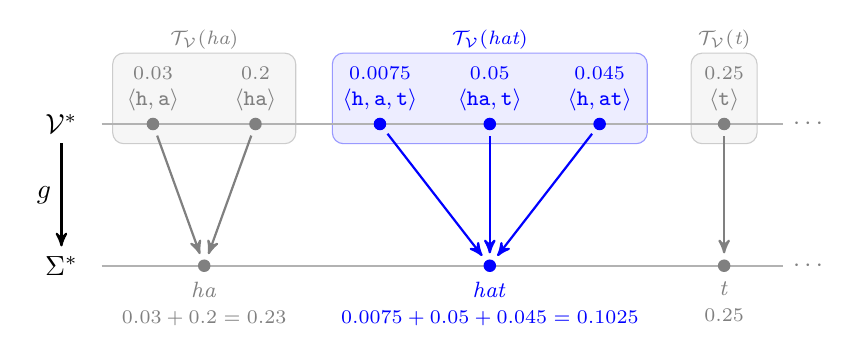
\begin{tikzpicture}[x=0.93cm]
  \colorlet{main}{blue}
  \colorlet{other}{black!50}
 
  % ---- preimages T_V(s) (drawn first so they sit behind) --------------------
  \draw[pf fibre=other, visible on=<2->] (0.15,1.55) rectangle (2.65,2.7);
  \draw[pf fibre=main,  visible on=<2->] (3.15,1.55) rectangle (7.45,2.7);
  \draw[pf fibre=other, visible on=<2->] (8.05,1.55) rectangle (8.95,2.7);
  \node[pf num=other, anchor=south, visible on=<2->] at (1.4,2.7)  {$\mathcal{T}_{\vocab}(\textit{ha})$};
  \node[pf num=main,  anchor=south, visible on=<2->] at (5.3,2.7)  {$\mathcal{T}_{\vocab}(\textit{hat})$};
  \node[pf num=other, anchor=south, visible on=<2->] at (8.5,2.7)  {$\mathcal{T}_{\vocab}(\textit{t})$};
 
  % ---- the two spaces -------------------------------------------------------
  \node (Vs) at (-0.55,1.8) {$\vocab^*$};
  \node (Ss) at (-0.55,0)   {$\Sigma^*$};
  \draw[->, thick] (Vs.south) -- node[left] {$g$} (Ss.north);
 
  \draw[thick, black!30] (0,1.8) -- (9.3,1.8) node[right, black!50, font=\small] {$\cdots$};
  \draw[thick, black!30] (0,0)   -- (9.3,0)   node[right, black!50, font=\small] {$\cdots$};
 
  % ---- token sequences with P(V = v; phi) -----------------------------------
  \node[pf pt=other] (v1) at (0.7,1.8) {};
  \node[pf seq=other] (v1l) at (v1.north) {$\langle \texttt{h}, \texttt{a} \rangle$};
  \node[pf num=other, anchor=south] at (v1l.north) {$0.03$};
 
  \node[pf pt=other] (v2) at (2.1,1.8) {};
  \node[pf seq=other] (v2l) at (v2.north) {$\langle \texttt{ha} \rangle$};
  \node[pf num=other, anchor=south] at (v2l.north) {$0.2$};
 
  \node[pf pt=main] (v3) at (3.8,1.8) {};
  \node[pf seq=main] (v3l) at (v3.north) {$\langle \texttt{h}, \texttt{a}, \texttt{t} \rangle$};
  \node[pf num=main, anchor=south] at (v3l.north) {$0.0075$};
 
  \node[pf pt=main] (v4) at (5.3,1.8) {};
  \node[pf seq=main] (v4l) at (v4.north) {$\langle \texttt{ha}, \texttt{t} \rangle$};
  \node[pf num=main, anchor=south] at (v4l.north) {$0.05$};
 
  \node[pf pt=main] (v5) at (6.8,1.8) {};
  \node[pf seq=main] (v5l) at (v5.north) {$\langle \texttt{h}, \texttt{at} \rangle$};
  \node[pf num=main, anchor=south] at (v5l.north) {$0.045$};
 
  \node[pf pt=other] (v6) at (8.5,1.8) {};
  \node[pf seq=other] (v6l) at (v6.north) {$\langle \texttt{t} \rangle$};
  \node[pf num=other, anchor=south] at (v6l.north) {$0.25$};
 
  % ---- strings --------------------------------------------------------------
  \node[pf pt=other] (s1) at (1.4,0) {};
  \node[font=\footnotesize, text=other, anchor=north] (s1l) at (s1.south) {\textit{ha}};
  \node[pf pt=main] (s2) at (5.3,0) {};
  \node[font=\footnotesize, text=main, anchor=north] (s2l) at (s2.south) {\textit{hat}};
  \node[pf pt=other] (s3) at (8.5,0) {};
  \node[font=\footnotesize, text=other, anchor=north] (s3l) at (s3.south) {\textit{t}};
 
  % ---- g: every token sequence goes to exactly one string -------------------
  \draw[pf map=other, visible on=<2->] (v1) -- (s1);
  \draw[pf map=other, visible on=<2->] (v2) -- (s1);
  \draw[pf map=main,  visible on=<2->] (v3) -- (s2);
  \draw[pf map=main,  visible on=<2->] (v4) -- (s2);
  \draw[pf map=main,  visible on=<2->] (v5) -- (s2);
  \draw[pf map=other, visible on=<2->] (v6) -- (s3);
 
  % ---- P(S = s; phi): mass collected from the preimage ----------------------
  \node[pf num=other, anchor=north, visible on=<3->] at (s1l.south) {$0.03 + 0.2 = 0.23$};
  \node[pf num=main,  anchor=north, visible on=<3->] at (s2l.south) {$0.0075 + 0.05 + 0.045 = 0.1025$};
  \node[pf num=other, anchor=north, visible on=<3->] at (s3l.south) {$0.25$};
\end{tikzpicture}
\end{center}
 
\vfill
 
\begin{itemize}
\item<2-> $g$ maps each token sequence to exactly one string
\item<2-> However, many token sequences can map to the same string $\mathbf{s}$: its preimage $\mathcal{T}_{\vocab}(\mathbf{s}) = g^{-1}(\mathbf{s})$
\item<3-> Each string collects the probability mass of its preimage:
\begin{equation*}
P(\mathbf{S} = \mathbf{s}; \probs) = \sum_{\mathbf{v} \in \mathcal{T}_{\vocab}(\mathbf{s})} P(\mathbf{V} = \mathbf{v}; \probs)
\end{equation*}
\end{itemize}
 
\vfill
 
\end{frame}


\begin{frame}{Example (Continued)}

\vfill

\begin{itemize}
\item Dividing by $P(\mathbf{S} = \textit{hat}; \probs)$ gives the posterior:
\begin{align*}
P(\mathbf{V} = \langle \texttt{h}, \texttt{a}, \texttt{t} \rangle \mid \mathbf{S} = \textit{hat}; \probs) &= 0.0075 / 0.1025 \approx 0.073\\
P(\mathbf{V} = \langle \texttt{ha}, \texttt{t} \rangle \mid \mathbf{S} = \textit{hat}; \probs) &= 0.05 / 0.1025 \approx 0.488\\
P(\mathbf{V} = \langle \texttt{h}, \texttt{at} \rangle \mid \mathbf{S} = \textit{hat}; \probs) &= 0.045 / 0.1025 \approx 0.439
\end{align*}
\item $\langle \texttt{h}, \texttt{a}, \texttt{t} \rangle$ gets little posterior mass, even though $\texttt{h}$ and $\texttt{t}$ are the two most probable tokens (a product of three probabilities is penalized relative to a product of two)
\item The ranking of the two-token segmentations comes down to $\phi_{\texttt{ha}}\phi_{\texttt{t}}$ vs.\ $\phi_{\texttt{h}}\phi_{\texttt{at}}$: increasing $\phi_{\texttt{at}}$ enough relative to $\phi_{\texttt{ha}}$ would flip it
\item The highest-posterior segmentation $\langle \texttt{ha}, \texttt{t} \rangle$ is the canonical tokenization $h(\textit{hat})$ from before
\end{itemize}

\vfill

\end{frame}


\begin{frame}{Unigram Inference}

\vfill

\begin{itemize}
\item For now, assume we know $\probs$ (or at least have estimates for it)
\item At inference time, Unigram tokenizes $\mathbf{s}$ by choosing the segmentation with the \textbf{highest posterior probability}:
\begin{align*}
h_{\probs}(\mathbf{s}) &= \operatorname*{arg\,max}_{\mathbf{v} \in \mathcal{T}_{\vocab}(\mathbf{s})} P(\mathbf{V} = \mathbf{v} \mid \mathbf{S} = \mathbf{s}; \probs)\\
&= \operatorname*{arg\,max}_{\mathbf{v} \in \mathcal{T}_{\vocab}(\mathbf{s})} \frac{P(\mathbf{V} = \mathbf{v}; \probs)}{P(\mathbf{S} = \mathbf{s}; \probs)}\\
&= \operatorname*{arg\,max}_{\mathbf{v} \in \mathcal{T}_{\vocab}(\mathbf{s})} P(\mathbf{V} = \mathbf{v}; \probs)\\
&= \operatorname*{arg\,max}_{\mathbf{v} \in \mathcal{T}_{\vocab}(\mathbf{s})} \prod_{t=1}^{|\mathbf{v}|} \phi_{v_t}
\end{align*}
\item Computed efficiently by a dynamic program (\textbf{Viterbi})
\end{itemize}

\vfill

\end{frame}


\begin{frame}{Example (Continued)}

\vfill

\begin{itemize}
\item With $\probs$ from before, $\langle \texttt{ha}, \texttt{t} \rangle$ has the highest probability ($0.05$ vs.\ $0.045$ and $0.0075$), so $h_{\probs}(\textit{hat}) = \langle \texttt{ha}, \texttt{t} \rangle$
\item Now swap the probabilities of $\texttt{t}$ and $\texttt{at}$: $\phi'_{\texttt{t}} = 0.15$, $\phi'_{\texttt{at}} = 0.25$, everything else unchanged
\begin{align*}
P(\mathbf{V} = \langle \texttt{h}, \texttt{a}, \texttt{t} \rangle; \probs') &= 0.3 \times 0.1 \times 0.15 = 0.0045\\
P(\mathbf{V} = \langle \texttt{ha}, \texttt{t} \rangle; \probs') &= 0.2 \times 0.15 = 0.03\\
P(\mathbf{V} = \langle \texttt{h}, \texttt{at} \rangle; \probs') &= 0.3 \times 0.25 = 0.075
\end{align*}
\item The Viterbi segmentation flips: $h_{\probs'}(\textit{hat}) = \langle \texttt{h}, \texttt{at} \rangle$
\end{itemize}

\vfill

\end{frame}

\begin{frame}{Unigram Training Basics}

\vfill

\begin{itemize}
\item Given a training corpus, we need to find $\vocab$ and $\probs$
\item \textbf{Top-down} approach: 
\begin{itemize}
\item We start with a large $\vocab$ (around 1M tokens, typically bytes/characters and all substrings up to some length)
\item $\probs$ initialized proportional to frequency in training corpus
\item Choice matters: if token is not in initial vocabulary, it will never be part of the tokenizer vocabulary!
\item We iteratively prune tokens until we reach the desired vocabulary size, while at the same time learning $\probs$
\end{itemize}
\item Core algorithm: \textbf{expectation-maximization (EM)}
\end{itemize}

\vfill

\end{frame}




\begin{frame}{Expectation-Maximization for Unigram}
 
\vfill
 
\begin{itemize}
\item Training Unigram is a chicken-and-egg problem:
  \begin{itemize}
  \item If we knew the segmentations, estimating $\probs$ would be easy
  \item If we knew $\probs$, we could infer the segmentations
  \end{itemize}
\item Expectation-maximization (EM) alternates between the two, starting from an initial guess $\probs^{(0)}$ (e.g., uniform):
  \begin{itemize}
  \item \textbf{E-step}: use the current $\probs^{(n)}$ to compute the posterior over segmentations of each string (``soft'' segmentations)
  \item \textbf{M-step}: re-estimate $\probs^{(n+1)}$ from these soft segmentations (count tokens weighted by their posterior, then normalize)
  \end{itemize}
\item Repeat until $\probs$ converges
\end{itemize}
 
\vfill
 
\end{frame}
 


\begin{frame}{Observed Data Log-Likelihood}
\begin{itemize}
\item We want to find the parameters $\probs$ that maximize the log-likelihood of our data (maximum likelihood estimation)
\item For a corpus $\mathcal{C} = \{ \mathbf{s}_i \}_{i=1}^K$, we compute the log-likelihood of the \textbf{observed data} as
\begin{align*}
\mathcal{L}(\mathcal{C}; \probs) &\overset{\text{def}}{=} \log \prod_{i=1}^{K} P(\mathbf{S} = \mathbf{s}_i; \probs)\\
&= \log \prod_{i=1}^{K} \sum_{\mathbf{v} \in \mathcal{T}_{\vocab}(\mathbf{s}_i)} P(\mathbf{V} = \mathbf{v}; \probs)\\
&= \sum_{i=1}^{K} \log \sum_{\mathbf{v} \in \mathcal{T}_{\vocab}(\mathbf{s}_i)} P(\mathbf{V} = \mathbf{v}; \probs)
\end{align*}
\item Optimizing $\mathcal{L}(\mathcal{C}; \probs)$ is difficult due to the log-sum structure
\end{itemize}

\end{frame}


\begin{frame}{Expected Complete Data Log-Likelihood}

\vfill

\begin{itemize}
\item If we include the latent segmentations $\mathbf{v}_i$, we have the \textbf{complete data} $\mathcal{X} = \{(\mathbf{s}_i, \mathbf{v}_i)\}_{i=1}^K$, whose log-likelihood is
\begin{align*}
\mathcal{L}(\mathcal{X}; \probs) &\overset{\text{def}}{=} \log \prod_{i=1}^{K} P(\mathbf{S} = \mathbf{s}_i, \mathbf{V} = \mathbf{v}_i; \probs)\\
&= \sum_{i=1}^{K} \log P(\mathbf{S} = \mathbf{s}_i, \mathbf{V} = \mathbf{v}_i; \probs)
\end{align*}
\item We cannot compute $\mathcal{L}(\mathcal{X}; \probs)$ ($\mathbf{v}_i$ is unknown), but we \emph{can} compute its expectation under the posterior with current parameters $\probs^{(n)}$:
\begin{align*}
&Q(\probs; \probs^{(n)}) \overset{\text{def}}{=} \sum_{i=1}^{K} \mathbb{E}_{\mathbf{v} \sim P(\mathbf{V} \mid \mathbf{S} = \mathbf{s}_i; \probs^{(n)})}\big[\log P(\mathbf{S} = \mathbf{s}_i, \mathbf{V} = \mathbf{v}; \probs)\big]\\
&\quad = \sum_{i=1}^{K} \sum_{\mathbf{v} \in \mathcal{T}_{\vocab}(\mathbf{s}_i)} \underbrace{P(\mathbf{V} = \mathbf{v} \mid \mathbf{S} = \mathbf{s}_i; \probs^{(n)})}_{\text{weights from current } \probs^{(n)}} \, \underbrace{\log P(\mathbf{V} = \mathbf{v}; \probs)}_{\text{increase by adjusting } \probs}
\end{align*}
\end{itemize}

\vfill

\end{frame}

\begin{frame}{Quick Recap}

\vfill 

\begin{itemize}
\item We want to optimize the observed data log-likelihood:
\begin{equation*}
\mathcal{L}(\mathcal{C}; \probs)= \sum_{i=1}^{K} \log \sum_{\mathbf{v} \in \mathcal{T}_{\vocab}(\mathbf{s}_i)} P(\mathbf{V} = \mathbf{v}; \probs)
\end{equation*}
\item Intuition: make \emph{corpus strings} more probable (where string probability is computed by marginalizing over valid segmentations)
\item We actually optimize the expected complete data log-likelihood:
\begin{equation*}
Q(\probs; \probs^{(n)}) = \sum_{i=1}^{K} \sum_{\mathbf{v} \in \mathcal{T}_{\vocab}(\mathbf{s}_i)} P(\mathbf{V} = \mathbf{v} \mid \mathbf{S} = \mathbf{s}_i; \probs^{(n)}) \log P(\mathbf{V} = \mathbf{v}; \probs)
\end{equation*}
\item Intuition: make \emph{valid segmentations} more probable, weighted by string frequency and current posterior
\end{itemize}

\vfill 

\end{frame}


\begin{frame}{How $Q$ Relates to $\mathcal{L}$}
 
\vfill
 
\begin{itemize}
\item It can be shown that $\mathcal{L}(\mathcal{C}; \probs)$ decomposes as follows:
\begin{align*}
\mathcal{L}(\mathcal{C}; \probs) &= Q(\probs; \probs^{(n)}) + \underbrace{\sum_{i=1}^{K} H(\mathbf{V} \mid \mathbf{S} = \mathbf{s}_i; \probs^{(n)})}_{\text{entropy: constant w.r.t.\ } \probs}\\
&\quad + \underbrace{\sum_{i=1}^{K} \operatorname{KL}\big(P(\mathbf{V} \mid \mathbf{S} = \mathbf{s}_i; \probs^{(n)}) \,\big\|\, P(\mathbf{V} \mid \mathbf{S} = \mathbf{s}_i; \probs)\big)}_{\geq 0;\ 0 \text{ at } \probs = \probs^{(n)}}
\end{align*}
\item The KL term is $0$ at $\probs^{(n)}$ and never negative, so pushing $Q$ up from $\probs^{(n)}$ also pushes $\mathcal{L}(\mathcal{C}; \probs)$ up, by at least as much
\item $Q$ plus the entropy term is known as the \textbf{evidence lower bound}
\end{itemize}
 
\vfill
 
\end{frame}
 
 
\begin{frame}{Intuition}
 
\vfill
 
\begin{center}
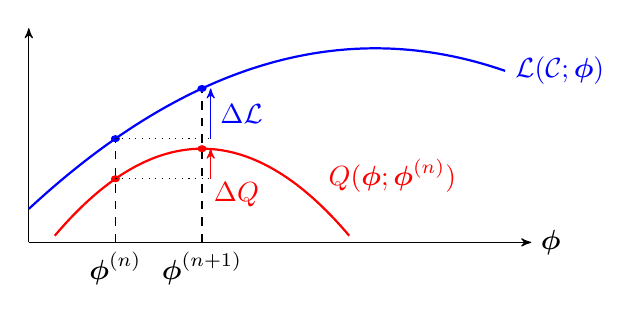
\begin{tikzpicture}[xscale=1.1, yscale=0.85]
  % axes
  \draw[->] (0,0) -- (5.8,0) node[right] {$\probs$};
  \draw[->] (0,0) -- (0,3.2);
  % observed-data log-likelihood
  \draw[thick, blue, domain=0:5.5, samples=80]
    plot (\x, {2.9 - 0.15*(\x-4)^2}) node[right] {$\mathcal{L}(\mathcal{C}; \probs)$};
  % Q = L - entropy - KL, built at phi^(n) = 1
  \draw[thick, red, domain=0.3:3.7, samples=80]
    plot (\x, {2.3 - 0.15*(\x-4)^2 - 0.3*(\x-1)^2});
  \node[red, anchor=west] at (3.35, 1.0) {$Q(\probs; \probs^{(n)})$};
  % current and next parameters
  \draw[dashed] (1,0) node[below] {$\probs^{(n)}$} -- (1,1.55);
  \draw[dashed] (2,0) node[below] {$\probs^{(n+1)}$} -- (2,2.3);
  \fill[red] (1,0.95) circle (1.5pt);
  \fill[blue] (1,1.55) circle (1.5pt);
  \fill[red] (2,1.4) circle (1.5pt);
  \fill[blue] (2,2.3) circle (1.5pt);
  % improvements
  \draw[dotted] (1,0.95) -- (2.15,0.95);
  \draw[dotted] (1,1.55) -- (2.15,1.55);
  \draw[->, red] (2.1,0.95) -- (2.1,1.4) node[pos=0, below right, inner sep=1pt] {$\Delta Q$};
  \draw[->, blue] (2.1,1.55) -- (2.1,2.3) node[midway, right] {$\Delta \mathcal{L}$};
\end{tikzpicture}
\end{center}
 
\begin{itemize}
\item The vertical gap between $\mathcal{L}$ and $Q$ at $\probs^{(n)}$ is the entropy term
\item Maximizing $Q$ moves us from $\probs^{(n)}$ to $\probs^{(n+1)}$
\item $\mathcal{L}(\mathcal{C}; \probs)$ rises by at least as much as $Q$: $\Delta\mathcal{L} \geq \Delta Q$
\item The difference between $\Delta \mathcal{L}$ and $\Delta Q$ is the KL term at $\probs^{(n+1)}$, which is $\geq 0$
\end{itemize}
 
\vfill
 
\end{frame}


\begin{frame}{E-Step}
 
\vfill
 
\begin{itemize}
\item Goal: compute the expected complete data log-likelihood under our current parameters, $Q(\probs; \probs^{(n)}) $
\item Defining a count function $c_v(\mathbf{v}) \overset{\text{def}}{=} \sum_{t=1}^{|\mathbf{v}|} \mathds{1}[v_t = v]$, we can write
\begin{equation*}
\log P(\mathbf{V} = \mathbf{v}; \probs)= \sum_{t=1}^{|\mathbf{v}|} \log \phi_{v_t} = \sum_{v \in \vocab} c_v(\mathbf{v}) \log \phi_v
\end{equation*}
\item Plugging this into $Q$ gives
\begin{equation*}
Q(\probs; \probs^{(n)}) = \sum_{v \in \vocab} \underbrace{\sum_{i=1}^{K} \smashoperator[r]{\sum_{\mathbf{v} \in \mathcal{T}_{\vocab}(\mathbf{s}_i)}} P(\mathbf{V} = \mathbf{v} \mid \mathbf{S} = \mathbf{s}_i; \probs^{(n)})\, c_v(\mathbf{v})}_{\hat{c}_v(\mathcal{C}; \probs^{(n)}):\ \text{expected count of } v \text{ in the corpus}} \log \phi_v
\end{equation*}
\item The E-step thus reduces to collecting these expected counts for all tokens in $\vocab$, which can be computed efficiently with the \textbf{forward-backward algorithm}
\end{itemize}
 
\vfill
 
\end{frame}
 
 
\begin{frame}{M-Step}
 
\vfill
 
\begin{itemize}
\item Goal: find the parameters that maximize $Q(\probs; \probs^{(n)})$, subject to the token probabilities summing to 1
\item Same as MLE for a categorical distribution, but with expected instead of observed counts:
\begin{equation*}
\phi^{(n+1)}_v = \frac{\hat{c}_v(\mathcal{C}; \probs^{(n)})}{\sum_{v' \in \vocab} \hat{c}_{v'}(\mathcal{C}; \probs^{(n)})}
\end{equation*}
\end{itemize}
 
\vfill
 
\end{frame}

\begin{frame}{Example (Continued)}
 
\vfill
 
\begin{itemize}
\item Corpus $\mathcal{C} = \{\textit{hat}\}$, uniform initialization $\phi^{(0)}_v = 0.2$ for all $v \in \vocab$
\item Segmentation probabilities and posteriors, where we use $P(\mathbf{S} = \textit{hat}; \probs^{(0)}) = 0.088$:
\begin{center}
\renewcommand{\arraystretch}{1.3}
\begin{tabular}{lcc}
$\mathbf{v}$ & $P(\mathbf{V} = \mathbf{v}; \probs^{(0)})$ & $P(\mathbf{V} = \mathbf{v} \mid \mathbf{S} = \textit{hat}; \probs^{(0)})$ \\
\hline
\rule{0pt}{2.8ex}$\langle \texttt{h}, \texttt{a}, \texttt{t} \rangle$ & $0.2^3 = 0.008$ & $1/11 \approx 0.091$ \\
$\langle \texttt{ha}, \texttt{t} \rangle$ & $0.2^2 = 0.04$ & $5/11 \approx 0.455$ \\
$\langle \texttt{h}, \texttt{at} \rangle$ & $0.2^2 = 0.04$ & $5/11 \approx 0.455$
\end{tabular}
\end{center}
\item For the expected counts, we weight each segmentation's token counts by its posterior, e.g.,
\begin{equation*}
\hat{c}_{\texttt{h}}(\mathcal{C}; \probs^{(0)}) = 1 \cdot \tfrac{1}{11} + 1 \cdot \tfrac{5}{11} = \tfrac{6}{11} \approx 0.545
\end{equation*}
\end{itemize}
 
\vfill
 
\end{frame}
 
 
\begin{frame}{Example (Continued)}
 
\vfill
 
\begin{itemize}
\item Normalizing the expected counts gives the new parameters:
\begin{center}
\renewcommand{\arraystretch}{1.3}
\begin{tabular}{lccccc}
 & \texttt{h} & \texttt{a} & \texttt{t} & \texttt{ha} & \texttt{at} \\
\hline
\rule{0pt}{2.8ex}$\phi^{(0)}_v$ & 0.2 & 0.2 & 0.2 & 0.2 & 0.2 \\
$\hat{c}_v(\mathcal{C}; \probs^{(0)})$ & 0.545 & 0.091 & 0.545 & 0.455 & 0.455 \\
$\phi^{(1)}_v$ & 0.261 & 0.043 & 0.261 & 0.217 & 0.217
\end{tabular}
\end{center}
\item $\texttt{a}$ only appears in the low-posterior segmentation $\langle \texttt{h}, \texttt{a}, \texttt{t} \rangle$, so its probability drops sharply
\item $\texttt{h}$ and $\texttt{t}$ gain the most: each appears in two segmentations, including a high-posterior one
\end{itemize}
 
\vfill
 
\end{frame}
 
\begin{frame}{Pruning}
 
\vfill
 
\begin{itemize}
\item EM alone does not change the vocabulary (it only re-estimates token probabilities over a fixed $\vocab$)
\item Every few EM iterations, remove a fraction of tokens (e.g., 20\%) and renormalize $\probs$, until the target size is reached
\item Remove the tokens whose removal lowers the expected complete data log-likelihood  the least ($\probs_{-v}$: $\probs$ without $v$, renormalized):
\begin{equation*}
L(v) = Q(\probs^{(n+1)}; \probs^{(n)}) - Q(\probs_{-v}^{(n+1)}; \probs^{(n)}_{-v})
\end{equation*}
\item Exact computation of $L(v)$ needs a forward-backward pass per token, so it is approximated: replace every use of $v$ by the best segmentation of its string without $v$
\end{itemize}
 
\vfill
 
\end{frame}


\begin{frame}{Empirical Comparison of BPE and Unigram}

\vfill

\begin{itemize}
\item Unigram results in segmentations that \textbf{align more closely with morphology} than BPE \citebutton{Hofmann et al.\ (2022)\cite{hofmann-etal-2022-embarrassingly}}{https://aclanthology.org/2022.acl-short.43/} 
\item This can lead to better performance \citebutton{Bostrom and Durrett (2020)\cite{bostrom-durrett-2020-byte}}{https://aclanthology.org/2020.findings-emnlp.414/} 
\end{itemize}

\medskip
\medskip

\centering

      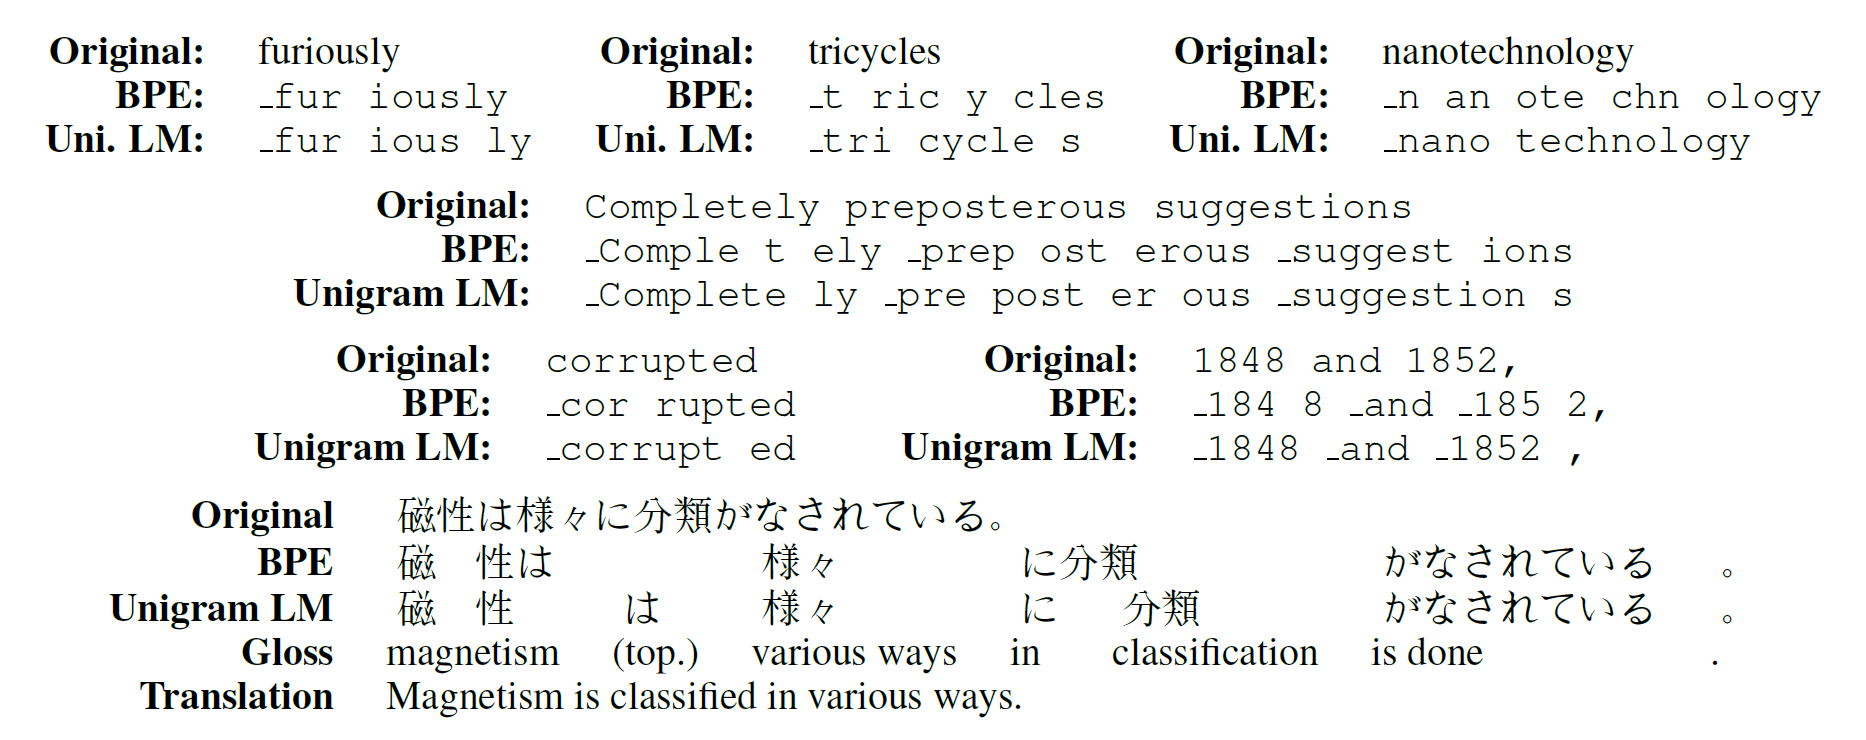
\includegraphics[width=0.9\textwidth]{figure/bostrom.png}

\vfill

\end{frame}


\section{Current Issues in Tokenization Research}

\begin{frame}{Tokenization and Interpretability}

\vfill

\begin{itemize}
\item Morphologically complex words (e.g., \textit{unhappiness}) tend to be segmented into several tokens by BPE and Unigram, but LLMs still ``understand'' their meaning as a whole
\item LLMs possess a \textbf{soft lexicon} encoded by the model weights that is much bigger than the \textbf{hard lexicon} defined by $\mathcal{V}$ 
\item The mapping between the hard and the soft lexicon is still poorly understood \citebutton{Kaplan et al.\ (2025)\cite{kaplan2025from}}{https://openreview.net/forum?id=328vch6tRs} 
\end{itemize}

\medskip
\medskip

\centering

      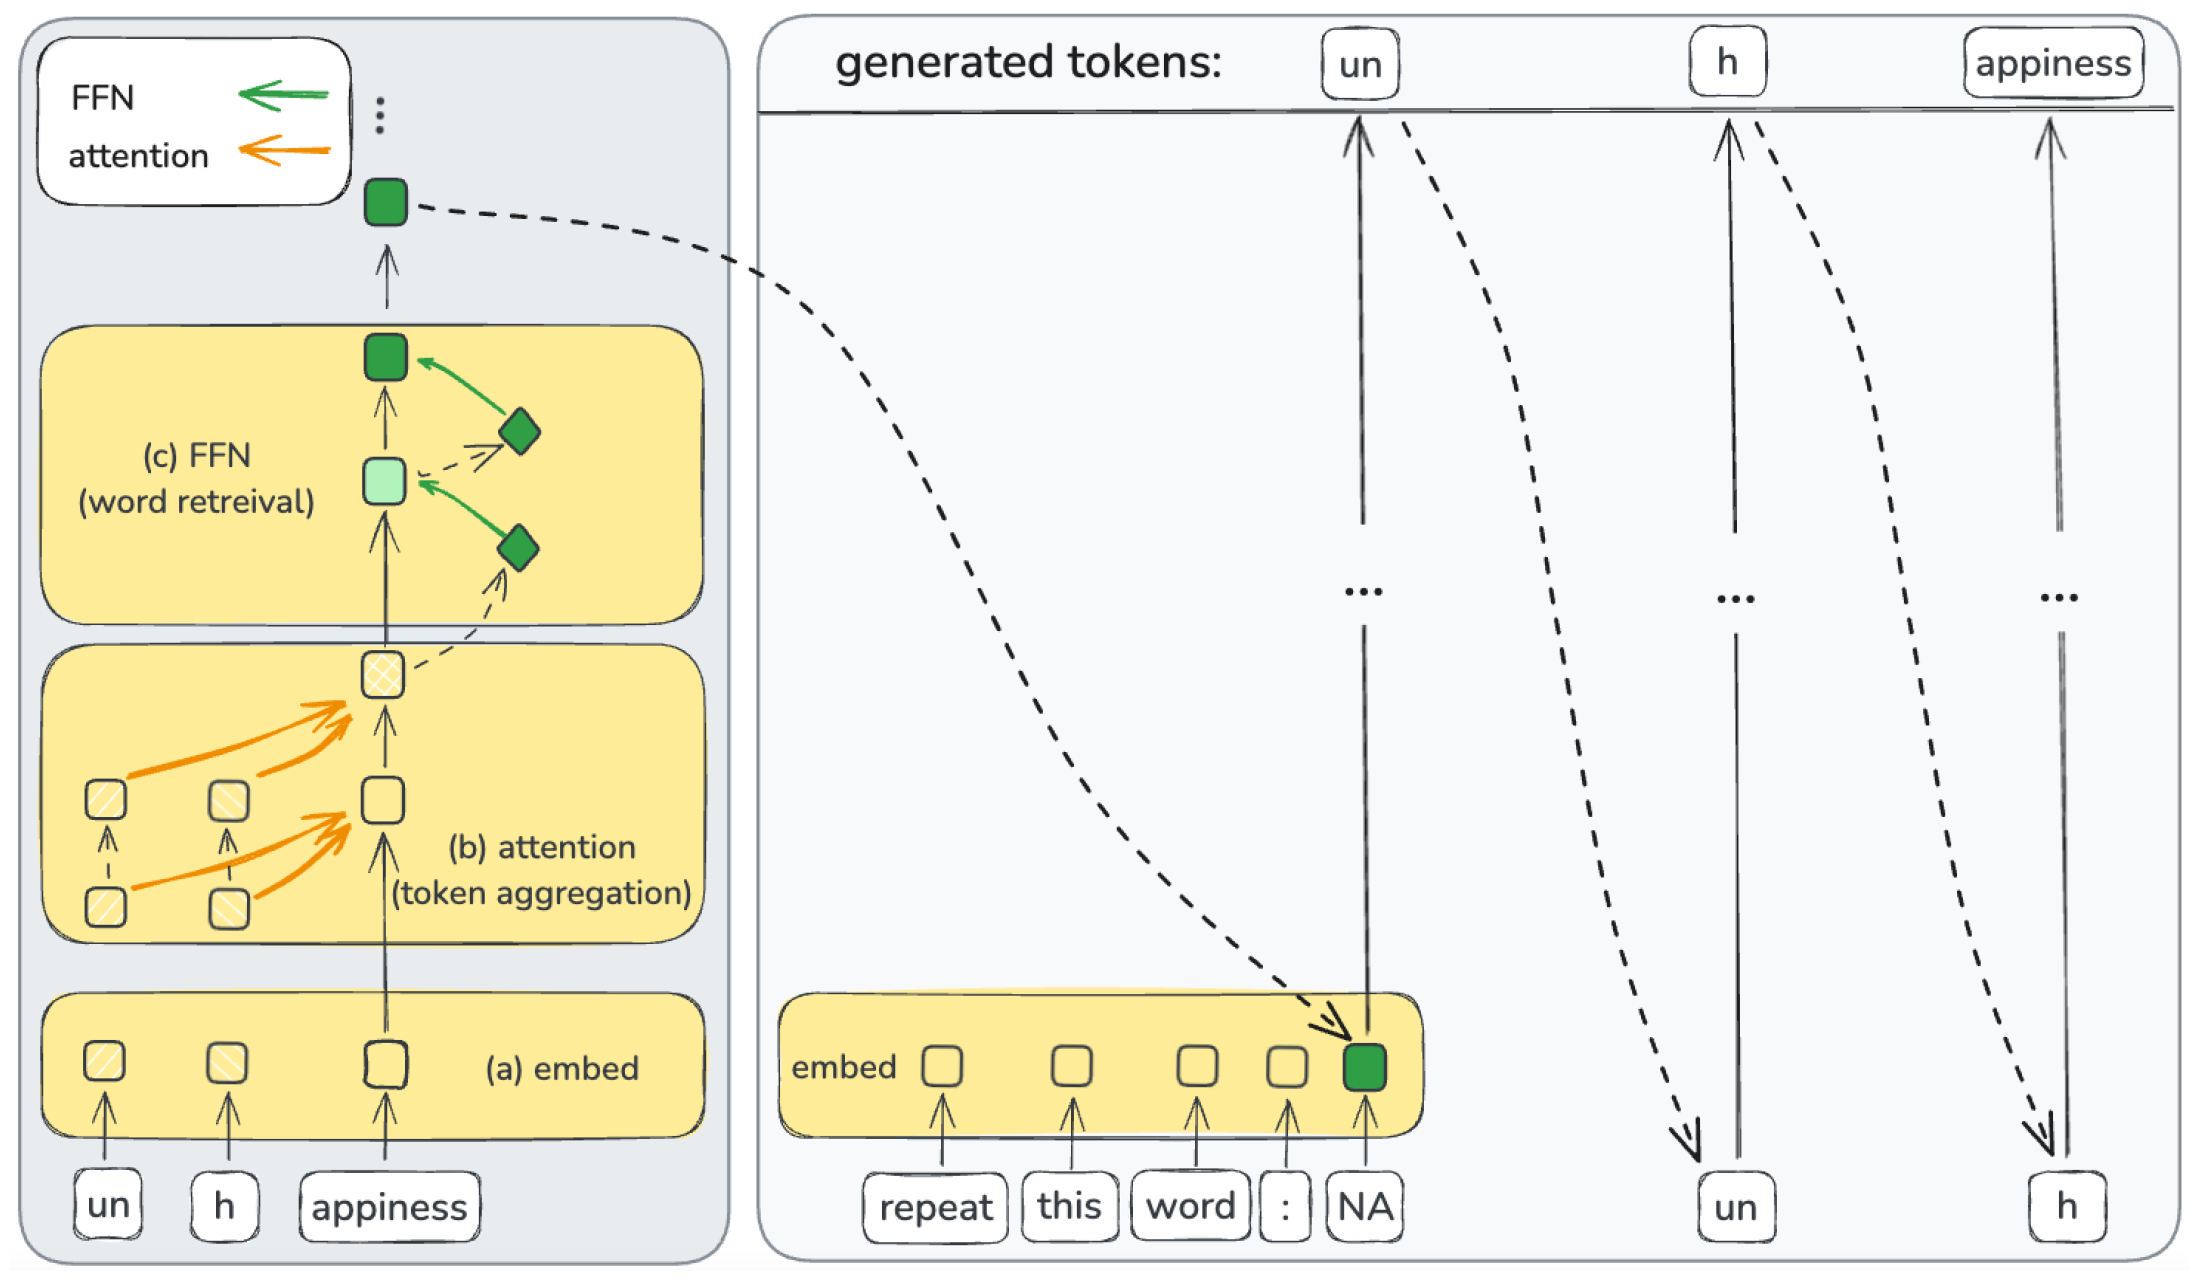
\includegraphics[width=0.5\textwidth]{figure/kaplan.png}

\vfill

\end{frame}


\begin{frame}{Multilingual Unfairness}

\vfill

\begin{itemize}
\item Tokenizers trained mostly on English data split the \emph{same} text into many more tokens in other languages, especially \textbf{low-resource languages} and \textbf{non-Latin scripts}
\item Longer sequences mean \textbf{higher costs}, \textbf{slower inference}, and less text fitting into the context window, which can \textbf{hurt downstream performance} \citebutton{Ahia et al.\ (2023)\cite{ahia-etal-2023-languages}}{https://aclanthology.org/2023.emnlp-main.614/} 
\end{itemize}

\medskip

\centering

      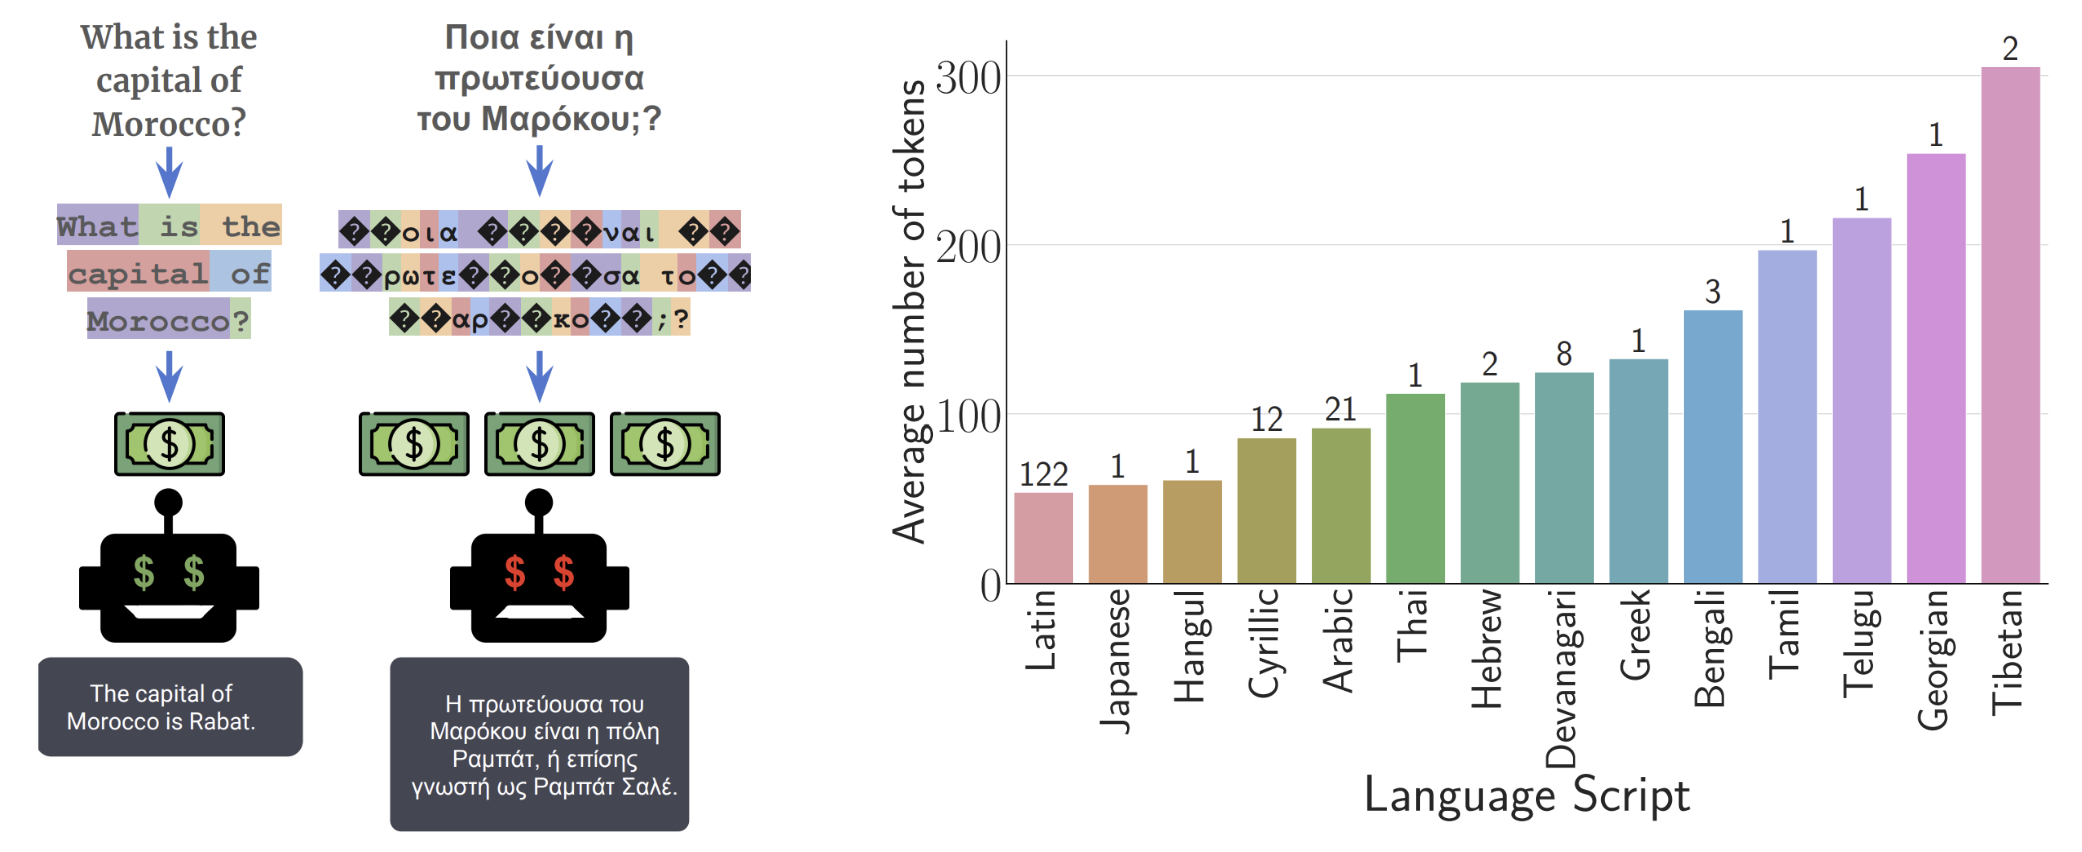
\includegraphics[width=0.9\textwidth]{figure/ahia.png}

\vfill

\end{frame}



\begin{frame}{Glitch Tokens}

\vfill

\begin{itemize}
\item The tokenizer training data can differ from the LLM training data
\item This can lead to undertrained tokens with unwanted behavior, so-called \textbf{glitch tokens} \citebutton{Land and Bartolo (2024)\cite{land-bartolo-2024-fishing}}{https://aclanthology.org/2024.emnlp-main.649/} 
\end{itemize}

\medskip
\medskip
\medskip


\centering

      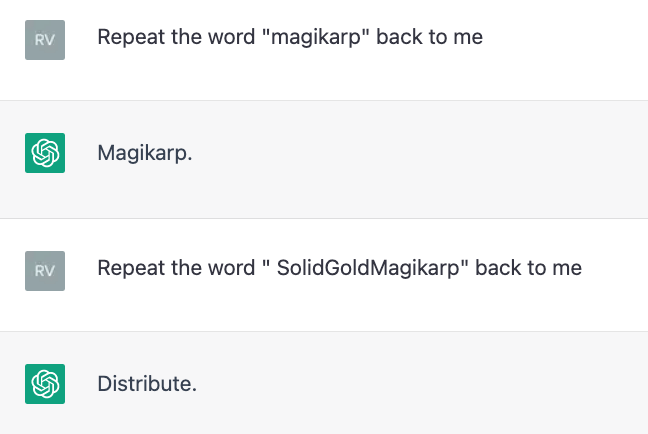
\includegraphics[width=0.5\textwidth]{figure/glitch.png}

\vfill
\end{frame}


\begin{frame}

\vfill

\centering \Large \bf Can we dispense with the tokenizer altogether?\\
\medskip
\medskip
Stay tuned for week 5!

\vfill
\end{frame}

% ==============================================================================

\begin{frame}[allowframebreaks,noframenumbering,plain]{References}
        \tiny
        \bibliographystyle{plain} %apalike
        \bibliography{refs-tokenization}
\end{frame}

\endlecture
\end{document}
